\chapter[Appendix 1]{Appendix 1 (supplementary to Chapter 2)}

\begin{table}[ht]
\tiny
\centering
\caption[Locations and characteristics of field sites.]{\small{Locations and characteristics of field sites. Hydrological class refers to the classification by Kennard et al. (2010).}}
\label{tab:Ch2sup_T1}
{\tabulinesep=1.2mm
\begin{tabu}to \textwidth {m{4cm}XXm{5cm}}
\hline
\texit{Site} & \texit{Longitude} & \texit{Latitude} & \texit{Hydrological class} \\
\hline
Snowy Creek & 147.413 & -36.569 & stable winter baseflow \\
Gibbo River & 147.709 & -36.756 & stable winter baseflow \\
Goodradigbee River & 147.826 & -36.444 & stable winter baseflow \\
Nariel Creek & 148.731 & -36.421 & stable winter baseflow \\
Jacob’s River & 148.427 & -36.727 & stable winter baseflow \\
Tuross River at Belowra & 149.709 & -36.201 & unpredictable baseflow \\
Genoa River & 149.321 & -37.174 & unpredictable baseflow \\
Wallagaraugh River & 149.714 & -37.371 & unpredictable baseflow \\
Mann River & 152.105 & -29.695 & unpredictable baseflow \\
Cataract Creek & 152.217 & -28.934 & unpredictable baseflow \\
Jilliby Creek & 151.389 & -33.246 & unpredictable intermittent \\
Sportsmans Creek & 142.981 & -29.467 & unpredictable intermittent \\
Mammy Johnsons River & 151.979 & -32.244 & unpredictable intermittent \\
Wadbilliga River & 149.694 & -36.259 & unpredictable intermittent \\
Tuross River downstream of Wadbilliga junction & 149.761 & -36.197 & unpredictable intermittent \\ \hline
\end{tabu}}
\end{table}
\noindent{\tiny{Kennard, M.J., Pusey, B.J., Olden, J.D., Mackay, S.J., Stein, J.L. & Marsh, N. (2010) Classification of natural flow regimes in Australia to support environmental flow management. \textit{Freshwater Biology}, 55, 171–193.}}
\clearpage

\begin{table}[ht]
\tiny
\centering
\caption[Summary of PCA across all hydrological metrics.]{\small{Summary for Principal Components Analysis across all 24 hydrological metrics described in this study. PC1 here corresponds to the first principal component of variation across metrics which had significant relationships with CWM wood density (Pearson's r = 0.990) (see Fig. \ref{figCh2_F4} in the main text for reference).}}
\label{tab:Ch2sup_T2}
{\tabulinesep=1.2mm
\begin{tabu}to \textwidth {m{4cm}XXXXX}
\hline
                       &  \texit{PC1}    & \texit{PC2}   & \texit{PC3}   & \texit{PC4}   & \texit{PC5} \\ \hline
Standard deviation     & 3.61  & 1.86  & 1.52  & 1.39  & 1.04  \\
Proportion of variance & 0.543 & 0.144 & 0.096 & 0.080 & 0.045 \\
Cumulative proportion  & 0.543 & 0.688 & 0.783 & 0.864 & 0.909 \\
\hline
\end{tabu}}
\end{table}
\clearpage

\begin{landscape}
\begin{table}[ht]
\tiny
\centering
\caption[Summary of PCA across all hydrological metrics.]{\small{Data density of trait dataset using (a.) site-specific field-sampled values for wood density only; (b.) site-specific field-sampled values combined with averaged values from other sites, and; (c.) (a) and (b) combined with values from wood density databases. For one species (\textit{Eucalyptus camphora subsp. humeana}), intraspecific variability was greater than 0.1 g / cm\textsuperscript{3}, and the averaged value was deemed not to be representative of the true value. This species was present at 1.4 \% cover at site 9.}}
\label{tab:Ch2sup_T4}
{\tabulinesep=1.2mm
\begin{tabu}to \linewidth {m{1.5cm}XXXXXX}
\hline
\textit{Site} & \textit{\# species sampled in field} (a) & \textit{Data density using field sampled values (a)} & \textit{\# species sampled in field at any site (b)} & \textit{Data density using field sampled values at any site (b)} & \textit{\# species with available trait values (c)} & \textit{Data density using all values (c)} \\ \hline
1 & 7 & 0.98 & 7 & 0.98 & 9 & 1.00 \\
2 & 1 & 1.00 & 1 & 1.00 & 1 & 1.00 \\
3 & 4 & 0.97 & 5 & 1.00 & 5 & 1.00 \\
4 & 4 & 0.81 & 5 & 0.95 & 6 & 0.97 \\
5 & 5 & 1.00 & 5 & 1.00 & 5 & 1.00 \\
6 & 5 & 1.00 & 5 & 1.00 & 5 & 1.00 \\
7 & 4 & 0.92 & 5 & 0.94 & 5 & 0.94 \\
8 & 7 & 0.98 & 8 & 1.00 & 8 & 1.00 \\
9 & 3 & 0.63 & 5 & 0.70 & 8 & 0.84 \\
10 & 3 & 0.64 & 6 & 0.97 & 6 & 0.97 \\
11 & 4 & 1.00 & 4 & 1.00 & 4 & 1.00 \\
12 & 3 & 0.62 & 6 & 0.88 & 8 & 0.98 \\
13 & 8 & 0.92 & 9 & 0.95 & 12 & 1.00 \\
14 & 4 & 0.75 & 5 & 0.80 & 8 & 0.86 \\
15 & 5 & 0.92 & 5 & 0.92 & 6 & 1.00 \\
\hline
\end{tabu}}
\end{table}
\end{landscape}
\clearpage

\begin{table}[ht]
\tiny
\centering
\caption[Sources of wood trait values for species which could not be sampled in the field.]{\small{Sources of wood trait values for species which could not be sampled in the field.}}
\label{tab:Ch2sup_T5}
{\tabulinesep=1.2mm
\begin{tabu}to \textwidth {XX}
\hline
\textit{Species} & \textit{Source of wood density value} \\ \hline
\textit{Guioa semiglauca} & Kooyman \& Westoby (2009) \\
\textit{Pittosporum spinescens} & Stuart (2011) \\
\textit{Cassinia trinerva} & Tng \& Bowman (2013) \\
\textit{Bedfordia arborescens} & Tng \& Bowman (2013) \\
\textit{Prostanthera lasianthos} & Tng \& Bowman (2013) \\
\textit{Pultenaea juniperina} & Tng \& Bowman (2013) \\
\textit{Ligustrum sinense} & Martínez-Cabrera et al. (2009) \\
\textit{Grevillea robusta} & Chave et al. (2009) - averaged value \\
\textit{Notelaea longifolia} & Chave et al. (2009) \\
\textit{Trema tomentosa subsp. aspera} & Chave et al. (2009) - averaged value \\
\hline
\end{tabu}}
\end{table}
\noindent{\tiny{Chave, J., Coomes, D., Jansen, S., Lewis, S.L., Swenson, N.G. \& Zanne, A.E. (2009) Towards a worldwide wood economics spectrum. \textit{Ecology Letters}, 12, 351–366.\newline
Kooyman, R.M. \& Westoby, M. (2009) Costs of height gain in rainforest saplings: Main-stem scaling, functional traits and strategy variation across 75 species. \textit{Annals of Botany}, 104, 987–993.\newline
Martínez-Cabrera, H.I., Jones, C.S., Espino, S. \& Schenk, H.J. (2009) Wood anatomy and wood density in shrubs: Responses to varying aridity along transcontinental transects. \textit{American Journal of Botany}, 96, 1388–1398.\newline
Stuart, S.A. (2011) Cold Comfort: Diversification and Adaptive Evolution across Latitudinal Gradients, \textit{PhD Thesis}.\newline
Tng, D.Y.P., Jordan, G.J. \& Bowman, D.M.J.S. (2013) Plant traits demonstrate that temperate and tropical giant eucalypt forests are ecologically convergent with rainforest not savanna. \textit{PLoS ONE}, 8, 1–13.}}

\clearpage


%%%% FIGURE 1
\begin{figure}[ht]
\begin{center}
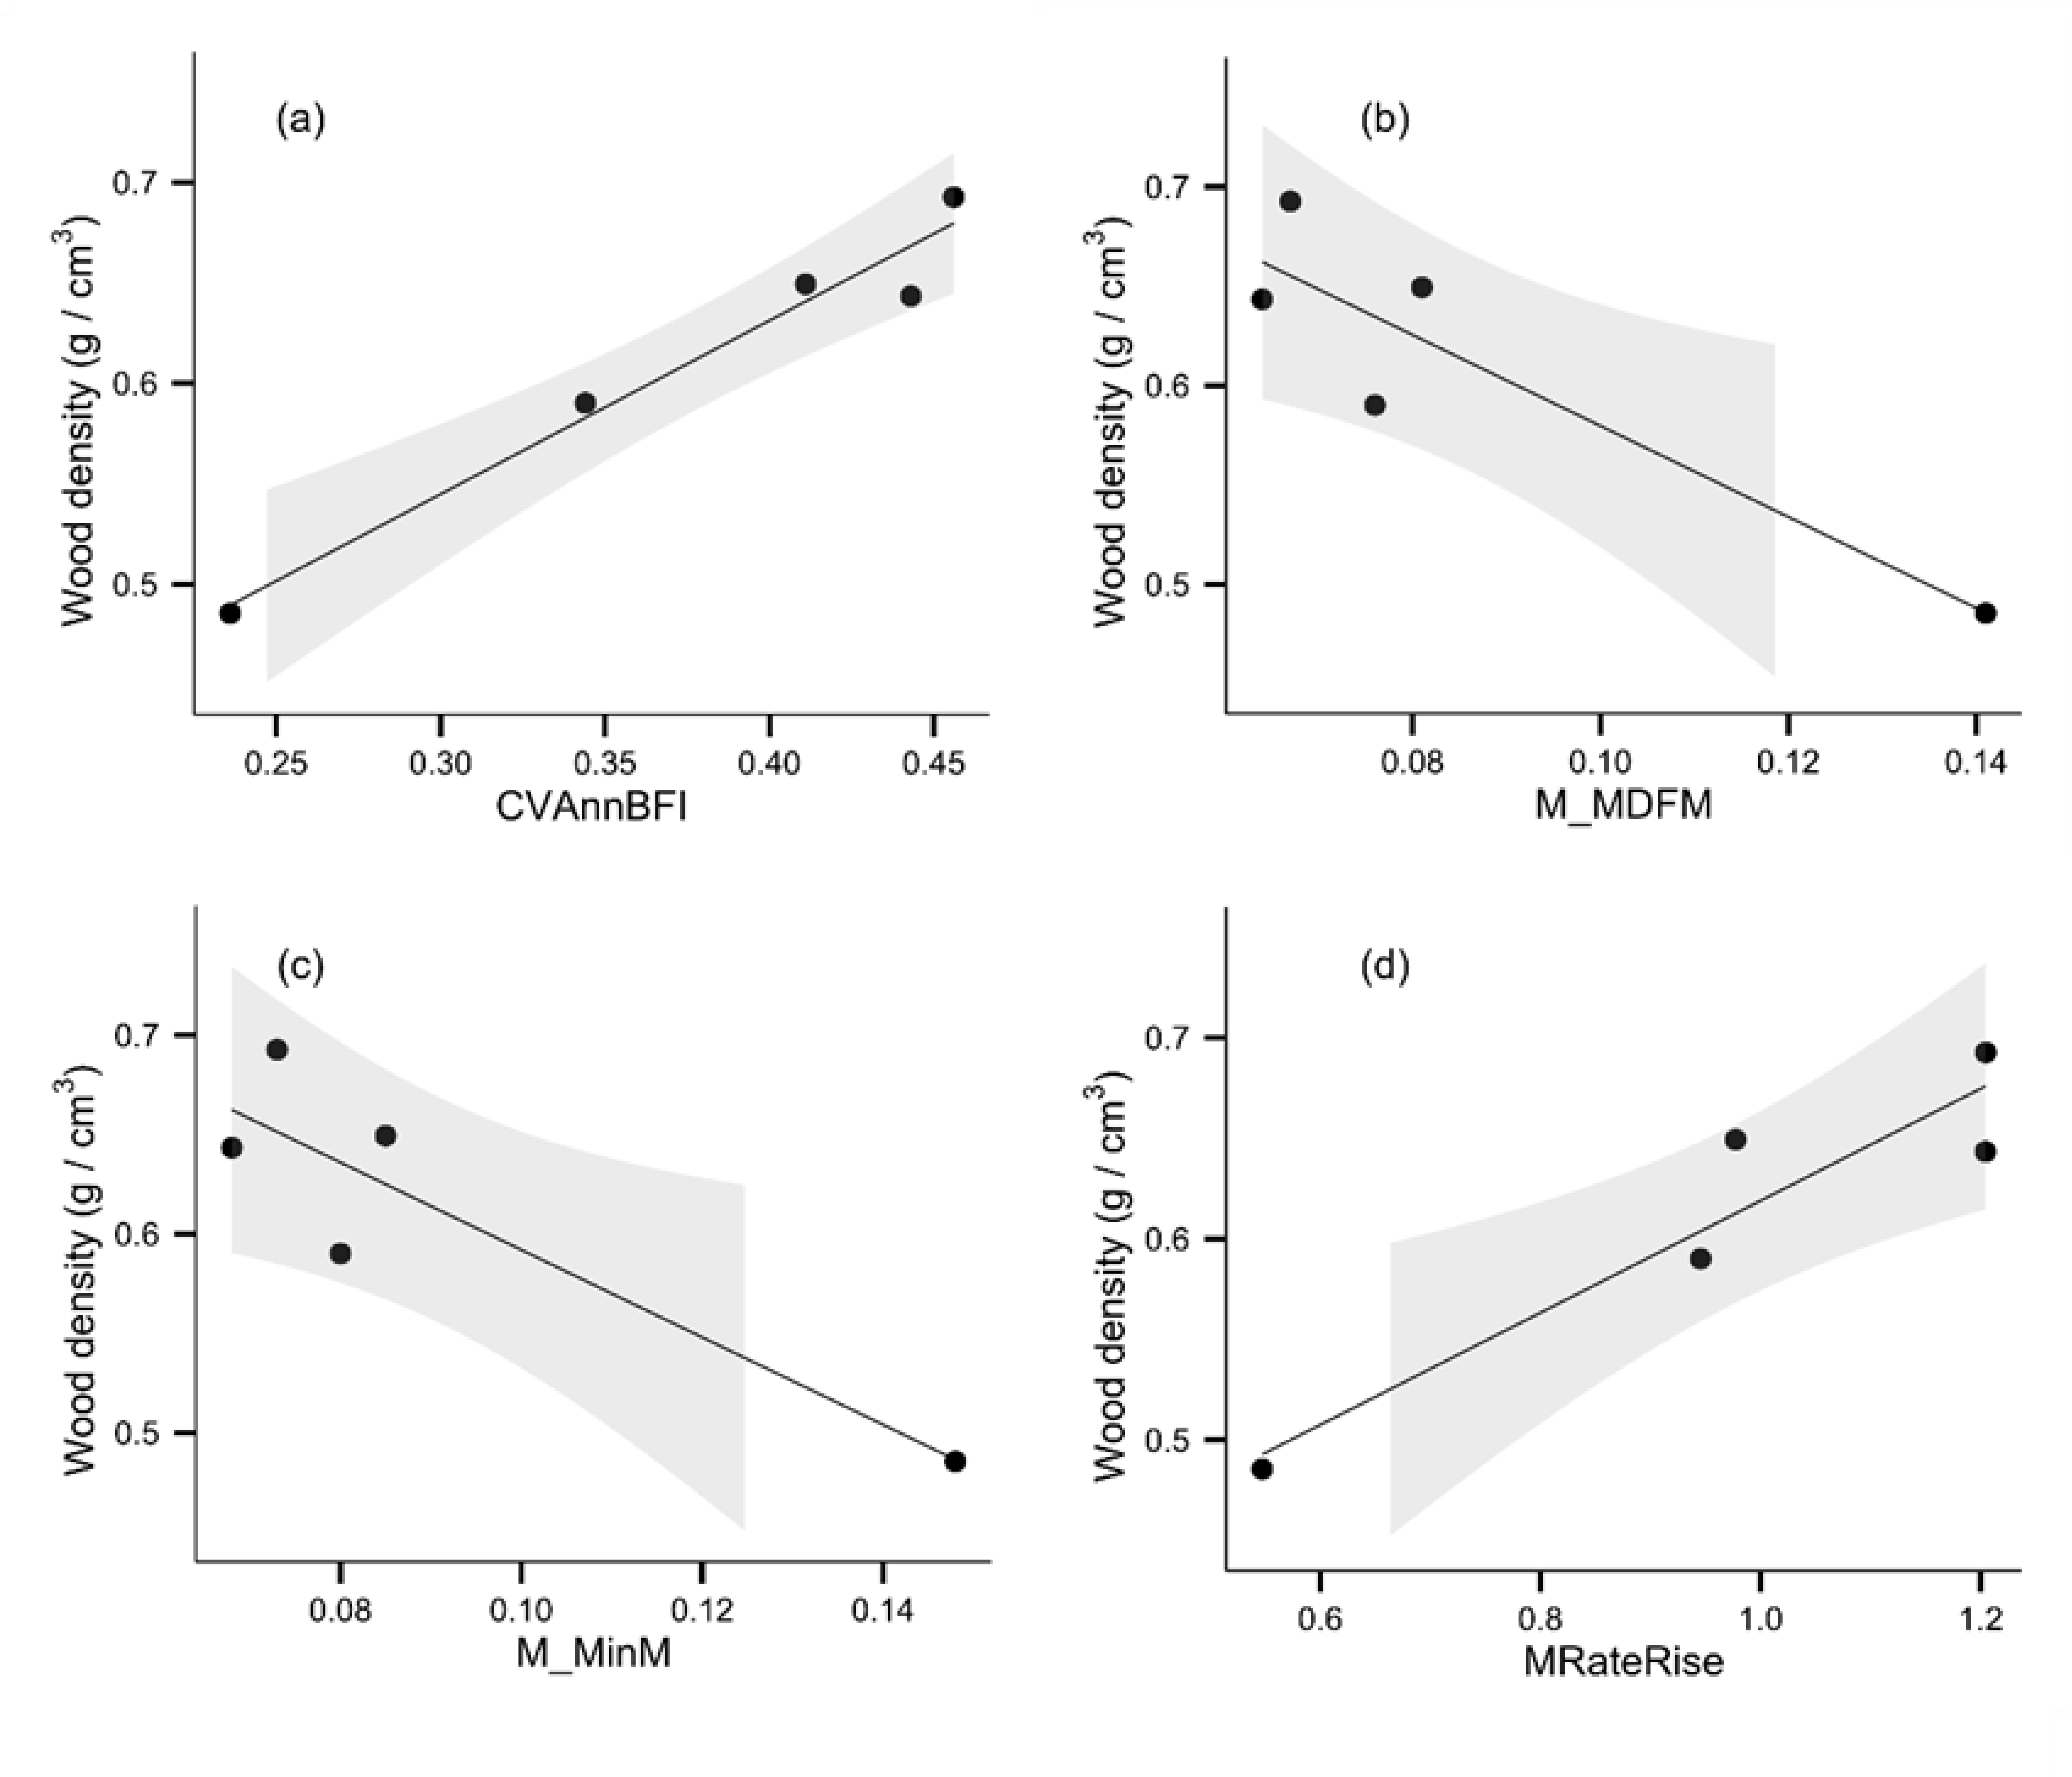
\includegraphics[width=\textwidth,keepaspectratio=true]{Ch2figS1.png} % figures can be in pdf, png, jpeg or eps format
\caption[Relationships between wood density of \textit{Casuarina cunninghamiana} and hydrological metrics]{\small{Relationships between wood density of \textit{Casuarina cunninghamiana} and hydrological metrics describing a.) interannual variability in baseflow index (CVAnnBFI) (R\textsuperscript{2} = 0.963 , P = 0.003); b.) contingency of monthly mean daily flow (M\_MDFM) (R\textsuperscript{2} = 0.826 , P = 0.033 ); c.) contingency of monthly minimum daily flow (M\_MinM) (R\textsuperscript{2} = 0.812 , P = 0.037 );  d.) mean flood rise rate (MRateRise)) (R\textsuperscript{2} = 0.885, P = 0.017). Shaded areas depict the 95 \% confidence interval around the regression model.}}
\label{Ch2sup_F1} % label for cross-referencing
\end{center}
\end{figure}   
\clearpage